\documentclass[openany]{article}

%Typesetting and language
\usepackage[american]{babel}
\usepackage[T1]{fontenc}
\usepackage{charter}
\usepackage{enumitem}
\usepackage{hyperref}

%Symbols
\usepackage{amssymb, amsmath, amsthm, bm}
\usepackage{mathrsfs}
\usepackage{mathtools}
\usepackage{marvosym}
\usepackage{MnSymbol}

%Colors & graphics
\usepackage[dvipsnames]{xcolor}
\usepackage{pgfplots}
\usepackage[numbered,framed]{matlab-prettifier}
\usepackage{pgfplots}
\usepackage{listings}
\usepackage{tikz}
\usetikzlibrary{arrows.meta}
\usepackage[object=vectorian]{pgfornament}
\usepackage{wrapfig}
\usepackage{varwidth}
\usepackage[framemethod=TikZ]{mdframed}
\usepackage{caption}
\usepackage{float}
\usepackage{geometry}
\usepackage{ulem}
\usepackage[most]{tcolorbox}
\usepackage{array}

\setlength{\parindent}{0pt}

\makeatletter
\g@addto@macro\bfseries{\boldmath}
\makeatother


\renewcommand{\Re}{\mathfrak{Re}}
\renewcommand{\Im}{\mathfrak{Im}}

\geometry{left=2cm,right=2cm,bottom=2cm,top=2cm}

\usepackage{fancyhdr}
\pagestyle{fancy}
\fancyhf{}
\renewcommand{\sectionmark}[1]{\markright{\arabic{section} - #1}}
\cfoot{\thepage}
\lhead{CS270}
\chead{HW5}
\rhead{Adam Yang}
\renewcommand{\headrulewidth}{1pt}


\DeclareMathOperator{\sgn}{sgn}
\DeclareMathOperator{\im}{im}
\DeclareMathOperator{\var}{var}
\DeclareMathOperator{\Orb}{Orb}
\DeclareMathOperator{\Fix}{Fix}
\DeclareMathOperator{\Stab}{Stab}
\DeclareMathOperator{\cov}{cov}
\DeclareMathOperator*{\esssup}{ess\,sup}
\DeclareMathOperator{\corr}{corr}
\DeclareMathOperator{\lik}{lik}
\DeclareMathOperator*{\argmin}{argmin}
\DeclareMathOperator*{\argmax}{argmax}

\newcommand{\niceline}[2]{%
		\nointerlineskip \vspace{.5\baselineskip}\hspace{\fill}
		{\color{#1}
				\resizebox{0.5\linewidth}{2ex}
				{{%
								{\begin{tikzpicture}
										\node  (C) at (0,0) {};
										\node (D) at (9,0) {};
										\path (C) to [ornament=#2] (D);
										\end{tikzpicture}}}}}%
		\hspace{\fill}
		\par\nointerlineskip \vspace{.5\baselineskip}
}

\definecolor{darkViolet}{HTML}{9400D3}
\newcommand{\sweetline}{%
		\noindent
		\begin{center}
				{\color{darkViolet}
						\resizebox{0.5\linewidth}{1ex}
						{{%
										{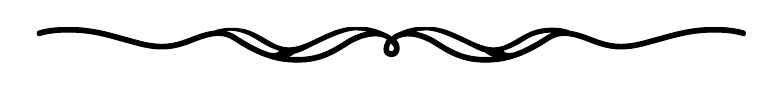
\begin{tikzpicture}
												\node  (C) at (0,0) {};
												\node (D) at (9,0) {};
												\path (C) to [ornament=85] (D);
												\end{tikzpicture}}}}}%
		\end{center}
}

\definecolor{remarkPurple}{HTML}{8346FF}
\definecolor{defBlue}{HTML}{0673FF}
\definecolor{exPurple}{HTML}{FF8710}

%THEOREM
\newtcbtheorem[auto counter,number within=section]{theorem}{Theorem}%
{enhanced,colback=white, breakable,frame empty,interior empty,colframe=cyan!50!white, top=8mm,
				coltitle=black,fonttitle=\bfseries,colbacktitle=cyan!15!white,
				borderline={0.5mm}{0mm}{cyan!15!white},
				borderline={0.5mm}{0mm}{cyan!50!white,dashed},
				attach boxed title to top left={yshift=-4mm},
				boxed title style={sharp corners=east,boxrule=1pt},varwidth boxed title}{thm}

%PROPOSITION
\newtcbtheorem[use counter from=theorem]{proposition}{Proposition}%
{enhanced,colback=white,breakable,frame empty,interior empty,colframe=defBlue!75!white, top=8mm,
				coltitle=black,fonttitle=\bfseries,colbacktitle=defBlue!20!white,
				borderline={0.5mm}{0mm}{defBlue!20!white},
				borderline={0.5mm}{0mm}{defBlue!50!white,dashed},
				attach boxed title to top left={yshift=-4mm},
				boxed title style={sharp corners=east,boxrule=1pt},varwidth boxed title}{prop}

%DEFINITION
\newtcbtheorem[use counter from=theorem]{definition}{Definition}%
{enhanced,colback=white,breakable,frame empty,interior empty,colframe=defBlue!75!white, top=8mm,
				coltitle=black,fonttitle=\bfseries,colbacktitle=defBlue!20!white,
				borderline={0.5mm}{0mm}{defBlue!20!white},
				borderline={0.5mm}{0mm}{defBlue!50!white,dashed},
				attach boxed title to top left={yshift=-4mm},
				boxed title style={sharp corners=east,boxrule=1pt},varwidth boxed title}{def}

%COROLLARY
\newtcbtheorem[use counter from=theorem]{corollary}{Corollary}%
{enhanced,colback=white,breakable,frame empty,interior empty,colframe=defBlue!75!white, top=8mm,
				coltitle=black,fonttitle=\bfseries,colbacktitle=defBlue!20!white,
				borderline={0.5mm}{0mm}{defBlue!20!white},
				borderline={0.5mm}{0mm}{defBlue!50!white,dashed},
				attach boxed title to top left={yshift=-4mm},
				boxed title style={sharp corners=east,boxrule=1pt},varwidth boxed title}{cor}

%REMARK
\newtcbtheorem[no counter]{remark}{Remark}%
{detach title, colback=white,enhanced ,breakable,frame empty, interior empty, fonttitle=\bfseries, coltitle=Violet, before upper={\tcbtitle.\quad},
				borderline west={0.5mm}{0mm}{remarkPurple!40!white},
				borderline west={0.5mm}{0mm}{remarkPurple!60!white,dashed}}{remark}

%LEMMA
\makeatletter
\newtcbtheorem[number within = tcb@cnt@theorem]{lemma}{Lemma}%
{enhanced,breakable,colback=white,frame empty,interior empty,colframe=orange!75!white, top=8mm,
				coltitle=black,fonttitle=\bfseries,colbacktitle=orange!20!white,
				borderline={0.5mm}{0mm}{orange!20!white},
				borderline={0.5mm}{0mm}{orange!50!white,dashed},
				attach boxed title to top left={yshift=-4mm},
				boxed title style={sharp corners=east,boxrule=1pt},varwidth boxed title}{lemma}
\makeatother


%PROOF
%%{enhanced,breakable,frame empty,interior empty,colframe=remarkPurple!75!white, top=8mm,
%	coltitle=black,fonttitle=\bfseries,colbacktitle=remarkPurple!20!white,
%	borderline={0.5mm}{0mm}{remarkPurple!20!white},
%	borderline={0.5mm}{0mm}{remarkPurple!50!white,dashed},
%	attach boxed title to top left={yshift=-4mm},
%	boxed title style={sharp corners=east,boxrule=1pt},varwidth boxed title}{prf}


\tcolorboxenvironment{proof}{% amsthm' 
				blanker,breakable,left=5mm,
				before skip=10pt,after skip=10pt,
				borderline west={0.5mm}{0pt}{cyan!40},
				borderline west={0.5mm}{0pt}{remarkPurple!10, dashed}}

%PROBLEM
\newtcbtheorem[auto counter]{problem}{Problem}%
{enhanced,breakable,colback=white,frame empty,interior empty,colframe=cyan!50!white, top=8mm,
				coltitle=black,fonttitle=\bfseries,colbacktitle=cyan!20!white,
				borderline={0.5mm}{0mm}{cyan!20!white},
				borderline={0.5mm}{0mm}{cyan!50!white,dashed},
				attach boxed title to top left={yshift=-4mm},
				boxed title style={sharp corners=east,boxrule=1pt},varwidth boxed title}{prob}

%EXAMPLE
%\newtcbtheorem[use counter from=problem]{example}{Example}%
%{enhanced,breakable,colback=white,frame empty,interior empty,colframe=remarkPurple!50!white, top=8mm,
%		coltitle=black,fonttitle=\bfseries,colbacktitle=remarkPurple!30!white,
%		borderline={0.5mm}{0mm}{remarkPurple!30!white},
%		borderline={0.5mm}{0mm}{remarkPurple!30!white,dashed},
%		attach boxed title to top left={yshift=-4mm},
%		boxed title style={sharp corners=east,boxrule=1pt},varwidth boxed title}{ex}


\newtcbtheorem[use counter from=theorem]{example}{Example}%
{detach title, colback=white,enhanced ,breakable,frame empty, interior empty, fonttitle=\bfseries, coltitle=black, before upper={\tcbtitle.\quad},
		borderline west={0.5mm}{0mm}{remarkPurple!30!white},
		borderline ={0.5mm}{0mm}{remarkPurple!30!white}}{example}

%SOLUTION
\newtcbtheorem[no counter]{solution}{Solution}%
{enhanced,breakable,colback=white,frame empty,interior empty,colframe=green!75!white, top=8mm,
				coltitle=black,fonttitle=\bfseries,colbacktitle=green!20!white,
				borderline={0.5mm}{0mm}{green!20!white},
				borderline={0.5mm}{0mm}{green!50!white,dashed},
				attach boxed title to top left={yshift=-4mm},
				boxed title style={sharp corners=east,boxrule=1pt},varwidth boxed title}{sol}
\definecolor{realPurple}{HTML}{AA05F9}
\definecolor{gray}{rgb}{0.5,0.5,0.5}
\definecolor{dkgreen}{rgb}{0,0.6,0}
\definecolor{mauve}{rgb}{0.58,0,0.82}

\lstset{frame=tb,
				style=Matlab-editor,
				language=C,
				aboveskip=3mm,
				belowskip=3mm,
				xleftmargin=3mm,
				showstringspaces=false,
				columns=flexible,
				frame=none,
				basicstyle={\small\ttfamily},
				numberstyle=\tiny\color{gray},
				keywordstyle=\color{blue},
				commentstyle=\color{dkgreen},
				stringstyle=\color{mauve},
				breaklines=true,
				breakatwhitespace=true,
				mlshowsectionrules = true,
				tabsize=3,
				backgroundcolor=\color{cyan!5}
}

\newcommand\mmybox[2][fill=cyan!20]{%
    \tikz[baseline]\node[%
        inner ysep=0pt, 
        inner xsep=2pt, 
        anchor=text, 
        rectangle, 
        rounded corners=1mm,
        #1] {\strut#2};%
}


\def\changemargin#1#2{\list{}{\rightmargin#2\leftmargin#1}\item[]}
\let\endchangemargin=\endlist

\linespread{1.4}



% MAIN DOC
\begin{document}

\title{HW 5}
\author{Adam Yang}
% \date{\today}
\maketitle




\section*{Problem1}

\subsection*{Algorithm}
\begin{proof}[Algorithm]{}
		\renewcommand{\qedsymbol}{}
		An Algorithm to calculate the sequence of die rolls gets to winning square as quickly as possible.
		\begin{lstlisting}[basicstyle=\fontsize{8}{9}\selectfont\ttfamily]
// this is a pseudo-code, for convenience we define add_roll() for vector<T> similar to push_back() in C++. It returns an original list added with a new square at the end and won't impact original list
// push_back() is simply C++ push_back() method for vector<T>
// reverse() is C++ STL one for vector, it takes O(n)
vector<int> findSeq( int[] d, int n ) //d[] is the input array of information, |d| = n+1, n is the last termination index
{
    // define infinity as the largest number we can get
    // define {infinity}.size() = infinity
    // won't use INT_MAX for convenience (overflowing issue)
    // here we denote the termination(last) index of d[] as n
    // if i is a ladder, d[i] = j, j>i (j is the termination of i)
    // if i is a chute, d[i] = infinity
    // if i is a normal square, d[i] = i
    // Will explain the code later
    if(n <= 6) return {n}; //trivially solved by rolling once to n
    vector<vector<int>> dp({}, n+1);
    //initialization
    for(int i = 1; n-i >= n-6; ++i){
        dp[i] = {n-i};
    }
    // start finding sequence
    for(int i = 7; n - i >= 0; ++i) {
        int min_index = -1;
        vector<int> min_seq = {infinity};
        // for some i, if d[i] = infinity, dp[infinity] = {infinity}
        // OPT(i) = min( 1 + OPT(d[i+r]) ), r = 1,2,...,6
        for(int s = i+1; s <= i+6; ++s){
            if(dp[d[s]].size() < min_seq.size()){
                min_index = s;
                min_seq = dp[d[s]];
            }
        }
        if(min_index == -1) {   //i+1:i+6 are all chute
            dp[i] = {infinity}
        } else {
            // min_index - i is the number we need to roll to get min_index, notice in this block min_index = 1,2,...,6
            dp[i] = min_seq.add_roll(min_index - i) // sequence is reverse order now, will reverse later
        }
    }
    return dp[0].reverse(); //if dp[0].size() == infinity, we can't reach n from n
}
		\end{lstlisting} 
\end{proof}



\begin{proof}[Explanation]{}
		\renewcommand{\qedsymbol}{} % hide the QED square
        I'll explain some variable used in pseudo-code above here

        \textbf{int[] d:} this is an input array that the problem provides, d[i] stores the information for each square, as explained from line 3 to 7
        
        \textbf{vector<vector<int>> dp:} this array needs n+1 elements since the map ranges from 0 to n. i $\in$ [0 , n], dp[i] stores the sequence with fewest times of rolls to reach n starting from i. (Prove later)
        
        \textbf{vector<T>.add\_roll():} this method add the new roll to the original vector. Return value and its general implementation is discussed in line 1.
        
        \textbf{return dp[0].reverse():} Since we always add a new roll to the end of the vector on line 30, we need to reverse to return a correct-order sequence
        
        \textbf{int min\_index, vector<int> min\_seq:} These are for finding and storing the sequence that takes least steps. From line 26 to 36, if there exists the sequence that takes minimum times of rolls out of 6, we update the sequence of roll for dp[i] with additional roll to min\_index (min\_index - i), else (all six chutes) we store \{$\infty$\} to denote it can't reach n as a starting point.
        
        \textit{Initialization:} \textbf{dp[n] = \{\}} because it takes no effort to reach n from n. \textbf{For i=n-6, n-5,..., n-1} we initialize dp[i] = \{n-i\} since we can reach n from i by rolling n-i = 1,2,...,6 once.

       
\end{proof}

\subsection*{Proof}
\begin{proof}[Correctness]{}
    For convenience, saying a sequence S is better than S' for square i means S takes less times of rolls to reach n than S' takes (|S| < |S'|). Optimal sequence S* for square i means S* takes fewest times of rolls to reach n starting from i than other sequence starting from i (i could be anything and won't matter since we start from i). We fix the size of input array d[] with size of n+1 and indexed from 0 to n.
    
\textbf{Goal:} Find the optimum sequence of roll to reach n starting from 0.

\textbf{Analysis:} Starting from i, we can roll once to reach i+s, s=1,2,...,6. Denotes (i+s)'s destination by d[i+s], d[i+s]$\geq$i+s>i. Rolling a dice to (i+s) will bring us to d[i+s], ($\infty$ if chute, i+s if normal square, i+s < k $\leq$ n if a ladder. Incur the times of roll from i to i+s 1. The sequence starting from d[i+s] to n to be *optimal*. The optimum does the best of six.
    
\textbf{Subproblem:}
    Starting from i, find the optimal sequence to reach n.
    
\textbf{Define:} Opt(i) to be the least times of roll to reach n starting from i. Opt($\infty$) := $\infty$ since there is no way to reach n.
    
\textbf{Recurrence Relation:}
    \texttt{Opt(i) = $\min_{s=1,2,...,6}$(1 + Opt( d[i+s] ) )}
    Notice that it is Opt(d[i+s]) instead of Opt(i+s). This is because whenever we roll a dice to a new square, it may lead us into three different situations. i+s could be a chute, a ladder, or a normal square and thus Opt(d[i+s]) can take their destination into consideration. If (i+s) is a chute, d[i+s] = $\infty$ > countable integer, meaning we won't choose to roll to a chute. If for some i$\in$[0,n-7], $\forall s = 1,2,...,6: $d[i+s] = $\infty$, there is no way square i could be a start point to reach n, thus Opt(i) = $\infty$. If (i+s) is not a chute, we will find the smallest of the Opt(d[i+s]) and add an additional roll to reach (i+s) as the sequence from d[i+s]>i to n to be optimal.
    
\textbf{Base Case:}
    \texttt{Opt(n) = 0, Opt(n-s) = 1, s = 1,2,...,6}
    
\textbf{Correctness Proof:}

    \textbf{To Prove:} dp[0].size() = Opt(0)
    
    We'll prove by strong induction on k
    
    \textbf{Base Case:} dp[n].size() = Opt(n) = 0; dp[n-1].size() = dp[n-2].size() = ... = dp[n-6].size() = Opt(n-1) = Opt(n-2) = ... = Opt(n-6)
    
    \textbf{Inductive Hypothesis:} for k=0,1,...,n-1, dp[n-k].size() = Opt(n-k). (n-k = n,n-1,...,1)
    
    \textbf{Inductive Step:} when k = n $\Rightarrow$ n-k = 0, the algorithm leads to
    \begin{center}
        \texttt{dp[0].size() = min$_{s=1,2,...,6}$( 1+ dp[ d[0+s] ].size() ) = min$_{s=1,2,...,6}$( 1+ Opt( d[0+s] ) )}
    \end{center}
    [by IH, because s=1,2,...,6: n-(k+s) $\leq$ n-1 when k = 0]

    (Although the algorithm assigns vector sequence to find the optimal sequence, since the times of rolls can be easily find through *.size()* method, finding the min times of rolls from i to n result in finding the optimal sequence from i to n)
    
    Therefore,
    \begin{center}
        \texttt{dp[0].size() = Opt(0)} [by Recurrence Relation]
    \end{center}
    
    So we find the fewest times of rolls to reach n from 0, and therefore find the optimal sequence by return dp[0].reverse(). If min times is $\infty$, we can't reach n. This completes the proof.

\end{proof}
\begin{proof}{Termination}
    Every for loop has a condition that is based of boundary upon a temporary variable. Notice that for all such temporary variables, there is no other assignment except for strictly increasing or decreasing based on the boundary. Therefore, the algorithm always terminates.
\end{proof}

\subsection*{Running Time}
\begin{proof}[Running Time]{Analyze the algorithm running time}
    	\renewcommand{\qedsymbol}{}
    	
    	From line 14-19, setting variables and assignment takes $\mathcal{O}(n)$ for the vector. From line 21 to 37, it takes $\mathcal{O}(n)$ for looping n-6 elements and $\mathcal{O}(1)$ assignment inside (line 26 to 31 simply find the smallest times of rolls among six elements, it takes $\mathcal{O}(1)$ for six elements). For the final reverse, it takes $\mathcal{O}(n)$
    	
    	Thus the running time $T(n)$ will be \[T(n)=3\mathcal{O}(n)=\mathcal{O}(n)\]
\end{proof}

\section*{Problem 2}

\subsection*{Algorithm}
\begin{proof}[Algorithm]{}
	An Algorithm to calculate the sequence of die rolls gets to winning square as quickly as possible.

I will use some ideas introduce in lecture, specifically edit distance. Denote size of string x as n, size of string y as m. Inserting k-length blanks to y is the same as k-length deletion in x ($1 \leq k \leq n $). Inserting k-length blanks to x is the same as k-length insertion in x ($1 \leq k \leq n $). Aligning two different characters means replacement. Notice that in this question, we can either insert/delete one blank at a time or insert/delete multiple blanks at a time.
		\renewcommand{\qedsymbol}{}
	
		\begin{lstlisting}[basicstyle=\fontsize{8}{9}\selectfont\ttfamily]
// this is a pseudo-code written to C++ like form for convenience
// push_back() and reverse() are C++ STL operation. reverse() takes O(n), push_back() takes O(1)
// string x,y are two words to compare, n = size of x, m = size of y
// A and c is the constant cost for insertion/deletion, B is the cost for replacement
vector<operation> findSeq( string x, string y, int n, int m, int A, int c, int B )
{
    define *operation* as a type that stores
    1. the type of operation and 2. the length of characters handles
    
    int dp[n+1][m+1]; // extra space of 0 base cases
    operation dp_op[n+1][m+1];
    //initialization
    dp[0][0] = 0; dp_op[0][0] = *doing nothing*;
    for(int i = 0; i <= n; ++i){
        dp[i][0] = min( A*i, A*c(i-1) );
        if( A*i < A*c(i-1) ) dp_op[i][0] = * turn length-i string into empty by deleting one by one *;
        else dp_op[i][0] = * turn length-i string into empty by deleting all i at the same time *;
    }
    for(int j = 0; j <= m; ++i){
        dp[0][j] = min( A*j, A*c(j-1) );
        if( A*i < A*c(j-1) ) dp_op[0][j] = * turn empty string into length-j string by inserting one by one *;
        else dp_op[0][j] = * turn empty string into length-j string by inserting all j at the same time *;
    }
    //start finding
    for(int i = 1; i <= n; ++i){
        for(int j = 1; j <= m; ++j){
            int min1 = infinity; int min2 = infinity;
            operation op1, op2, op3;
            // min dp[i-k,j]+A+c(k-1), k = 1,2,...,i
            for(int k1 = 1; k1 <= i; ++k){
                if( dp[i-k1][j] + A + c*(k-1) < min1 ){
                    min1 = dp[i-k1][j] + A + c*(k-1);
                    op1 = * x[i-k1+1:i] is aligned with k1 empty blanks insert k1 blanks to the end of y[j] *
                }
            }
            // min dp[i,j-k]+A+c(k-1), k = 1,2,...,j
            for(int k2 = 1; k2 <= j; ++k){
                if( dp[i][j-k2] + A + c*(k-1) < min2 ){
                    min2 = dp[i][j-k2] + A + c*(k-1);
                    op2 = * y[j-k2+1:j] is aligned with k2 empty blanks and insert k2 blanks to the end of x[i] *
                }
            }
            // dp[i-1][j-1] + B (1 if x[i] != x[j] else 0)
            if(x[i]==y[j]){
                min3 = dp[i-1][j-1];
                op3 = { x[i] is aligned with y[j], they are the same we do nothing }
            } else {
                min3 = dp[i-1][j-1] + B;
                op3 = { x[i] is aligned with y[j], replace x[i] to y[j] or y[j] to x[i] }
            }
            dp[i][j] = min( min1, min2, min3 );
            dp_op[i][j] = op1 if min1 is smallest, op2 if min2 is smallest, op3 if min3 is smallest
        }
    }
    //finding the sequence of operation
    vector<operation> res;
    int i = n; int j = m;
    while(i != 0 || j !=0){
        operation temp = dp_op[i][j];
        res.push_back(temp);
        if(temp does nothing or only replace one character){ --i; --j; }
        else{
            // we get dp[i][j] from dp[i-k1][j]
            if( temp operation inserts k1 blanks to y[j] ) i -= k1;
            // we get dp[i][j] from dp[i][j-k2]
            else j -= k2; //temp inserts k2 blanks to x[i]
        }
    }
    
    return res.reverse();
}
		\end{lstlisting} 
\end{proof}

\begin{proof}[Explanation]{}
		\renewcommand{\qedsymbol}{} % hide the QED square
        I'll explain some variable used in pseudo-code above here. i$\in$[0,n], j$\in$[0,m]

        \textbf{inputs:} Input parameters have been discussed in the code above
        
        \textbf{int[][] dp:} this is a 2d array with (n+1)*(m+1) for extra 0 base cases. dp[i][j] stores the minimum cost for aligning x[1,...,i], y[1,...,j].  Prove later.
        
        \textbf{operation[][] dp\_op} this is a 2d array with (n+1)*(m+1) for extra 0 base cases. dp\_op[i][j] stores the last operation in the cheapest sequence of operations to align x[1,...,i], y[1,...,j], $i,j\in[0,n]$. Since dp[i][j] is achieved from dp[i'][j'], i'+j' < i+j, the algorithm lead to dp\_op[i][j] storing the operation from aligning x[1...i'] and y[1...j'] to aligning x[1...i] and y[1...j]. If dp[i][j] indeed stores the min cost for alignment, dp\_op[i][j] stores the last operation in the optimal sequence operation. Therefore, as long as dp[i][j] finds the lowest cost for alignment $\Rightarrow$ dp[i][j] finds the best sequence of operations $\Rightarrow$ dp\_op[i][j] stores the last operation from the best sequence. Will prove dp[i][j]'s optimality later.
        
        \textbf{int min1, min2:} these are temporary values to help finding the cheapest operation from dp[i-k][j] or dp[i][j-k] + the cost for deleting k = 1 to k = i or j. Let's prove such a for loop indeed find the cheapest. WLOG, let's look at finding min1. The for loop from line 30 to 35 ends when k1 > i.
        
        \textbf{Prove: The for loop finds the min value}
        \begin{enumerate}
            \item[] \textbf{Loop Invariant:} At the end of iteration  k  of the loop, the variable min1 should contain the min of the values from dp[i-1][j]+A to dp[i-k][j]+A+c(k-1).
        
        \item[] \textbf{Initialization:} At the end of the loop the loop invariant states: 'At the end of the first iteration of the loop, the variable answer should contain the min of the values from dp[i-1][j]+A to dp[i-1][j]+A. The min of the values is dp[i-1][j]+A and this is what answer has been set to.
        
        \item[] \textbf{Maintenance:} Assume that the loop invariant holds at the end of iteration k' = k-1. Then it must be that answer contains the sum of values from dp[i-1][j]+A to dp[i-k+1][j]+A+c(k-2). In the body of the loop we assign dp[i-k''][j]+A+c, k'' $\leq$ k', to min1 if it's smaller than current min1. Thus at the end of iteration  k'+1=k, answer will contain the sum of value from dp[i-1][j]+A to dp[i-k][j]+A+c(k-1) by comparison, which is what we needed to prove.
        
        \item[] \textbf{Termination:} When the for-loop terminates  k'=k-1+1=k . Now the loop invariant gives: The variable answer contains the minimum of all values checked. This is exactly the value that the for loop should output, and which it then outputs. Therefore the for-loop is correct. Same for min2 and min3. $\square$
        \end{enumerate}

        \textbf{int min3:} this is a temporary value for finding the cost of operation for aligning x[i] and y[j]
        
        \textbf{vector<operation> res:} this is a the vector that stores the best sequence of operation in reverse order (we add the operation from back to front using push\_back()). Therefore, we need to reverse the order when we return
       
\end{proof}

\subsection*{Proof}
\begin{proof}[Correctness]{}
    We denote the size of string x as n, that of y as m. The cost of replacement B, the cost of inserting/deleting k characters A + c(k-1) where A and c are constants

    \textbf{Goal:} find the optimum way to insert blanks into both strings to minimize the alignment cost.
    
    \textbf{Explanation:} aligning x[$1...n$] with y[$1...m$] involves following $1+n+m$ cases:
    
    1. x[$n$] is aligned with y[$m$]; incur cost B * 1 if x[$n$] != y[$m$] else 0. x[$1...n-1$] with y[$1...m-1$] are aligned *optimally*.
    
    2. x[n-k$_1$+1:n] is aligned against a k$_1$-length blank: incur cost A+c(k$_1$-1). x[1..n-k$_1$] and y[1..m] are aligned *optimally*.
    
        \qquad 2.1 k$_1$=1, incur cost A. x[$1...n-1$] and y[$1...m$] are aligned *optimally*
        
        \qquad \vdots
        
        \qquad 2.n k$_1$ = $n$, incur cost A + c(n-1). x[0] and y[$1...m$] are aligned *optimally*
    
3. y[m-k$_2$+1:m] is aligned against a k$_2$-length blank: incur cost A+c(k$_2$-1). x[1..n] and y[1..m-k$_2$] are aligned *optimally*.

        \qquad 3.1 k$_2$=1, incur cost A. x[$1...n$] and y[$1...m-1$] are aligned *optimally*
        
        \qquad \vdots
        
        \qquad 3.n k$_1$ = $n$, incur cost A + c(m-1). x[$1...n$] and y[0] are aligned *optimally*

The optimum does the best of the $1+n+m$.

    \textbf{Subproblems:} optimal alignment of the first i characters of x ($0 \leq i \leq n$) and the first j characters of y ($0 \leq j \leq m$).
    
    \textbf{Define:} OPT(i,j) := to be the minimum total cost for aligning x[$1...i$] with y[$1...j$].
    
    \textbf{Recurrence Relation:} 
    \begin{center}
        \texttt{Opt(i,j) = min(  Opt(i-1,j-1) + B*( 1 if x[i]!=y[j] else 0 ),\\
        min$_{k_1=1,...,i}$( Opt(i-k$_1$,j) + A + c(k$_1$-1) ),\\
        min$_{k_2=1,...,j}$( Opt(i,j-k$_2$) + A + c(k$_2$-1) )  )}
    \end{center}
    
    (1) when x[i] aligns with y[j] and x[i] == y[j], we don't need to do anything, thus Opt(i,j) = Opt(i-1,j-1)
    
    (2) when x[i] aligns with y[j] and x[i] != y[j], we need to replace the last character, thus Opt(i,j) = Opt(i-1,j-1) + B
    
    (3) here comes the complicated part. when x[i] is aligned with k$_1$ blanks, we need to delete all k$_1$ blanks starting from x[i-k$_1$], thus Opt(i,j) = Opt(i-k$_1$,j)+A+c(k$_1$-1), k$_1\in$[1,i]. Since we need to find the lowest cost one, we take the minimum from all k$_1$=1,...,j situation
    
    (4) when y[j] is aligned with k$_2$ blanks, we need to insert all k$_2$ characters starting from y[j-k$_2$], thus Opt(i,j) = Opt(i,j-k$_2$)+A+c(k$_2$-1), k$_2\in$[1,j]. Since we need to find the lowest cost one, we take the minimum from all k$_2$=1,...,j situation
    
    Since we take the cheapest, we take the minimum from above situations.
    
   \textbf{Base cases:}
   \begin{center}
        \texttt{OPT(i,0) = min( A*i, A+c(i-1) ) [ turn length-i string into empty string]}
        
        \texttt{OPT(0,j) = min( A*j, A+c(j-1) ) [ turn empty string into length-j string]}
        
   \end{center}
   
        Notice that we either delete/insert one by one or everything as a whole. Lets prove why it is the case. WLOG, let's look a deletion, turn length-i string into empty string. In order to delete all i, we need kA + k'c cost in total, k$\in$[1,i], k'$\in$[0,i-1]. Notice that k+k' always equal i because we delete i-length string. 
        
        When A*i < A+c(i-1), A < c$\frac{i-1}{i-1} \Rightarrow A < c \Rightarrow$ A*i $\leq$ A*(i-c$_1$)+c(c$_1$), c$_1 \in$[1,n-1]. Thus A*i is still the cheapest.
        
        When A*i $\geq$ A+c(i-1), A $\geq$ c $\Rightarrow$ Ac$_2$ + c(i-c$_2$) $\geq$ A+c(i-1). Thus A+c(i-1) is still the cheapest. Therefore, either delete one by one or delete as a whole is cheapest. QED
        
        For insertion, it is simply the symmetric of deletion. Thus, either inserting one by one or inserting as a whole is cheapest. QED

    \textbf{Correctness Proof:}
    
    \textbf{To prove:} dp[n][m] = OPT(n,m)
    
    We will prove by induction on i+j, i$\in$[0,n], j$\in$[0,m].
    
    \textbf{Base Case:} i+j = 0 $\Rightarrow$ i = j = 0. dp[0][0] = 0 = Opt(0,0)
    
    \textbf{Inductive Hypothesis:} whenever 0 $\leq$ i'+j' < i+j, dp[i'][j'] = OPT(i',j'), i $\geq$ i', j $\geq$ j' $\geq$ 0
    
    \textbf{Inductive Step:} i'+j' = i+j (dp[i][j])
    
    \textbf{Inductive Case 1:}  x[i] == y[j], and i > 0 and j > 0:
    Algorithm writes 
    \begin{center}
        \texttt{dp[i][j] = min( dp[i-1][j-1], min$_{k_1=1,...,i}$( dp[i-k$_1$][j] + A + c*(k$_1$-1) ),\\min$_{k_2=1,...,j}$( dp[i][j-1] + A + c*(k$_2$-1) ) )\\
        = min ( OPT(i-1,j-1), min$_{k_1=1,...,i}$( OPT(i-$k_1$,j) + A + c(k$_1$-1) ), \\( by IH, because (i-1) + (j-1) < i+j, (i-k$_1$)+j < i+j, i+(j-k$-2$) < i+j, k$_1$$\in$[1,i], k$_2$$\in$[1,j] ) \\min$_{k_2=1,...,j}$( OPT(i,j-k$_2$) + A + c*(k$_2$-1) ) ) = Opt(i,j) \\( by recurrence relation )}
    \end{center}

    \textbf{Inductive Case 2:}  x[i] != y[j], and i > 0 and j > 0:
    Algorithm writes 
    \begin{center}
        \texttt{dp[i][j] = min( dp[i-1][j-1] + B, min$_{k_1=1,...,i}$( dp[i-k$_1$][j] + A + c*(k$_1$-1) ),\\min$_{k_2=1,...,j}$( dp[i][j-1] + A + c*(k$_2$-1) ) ) \\( by IH, because (i-1) + (j-1) < i+j, (i-k$_1$)+j < i+j, i+(j-k$-2$) < i+j, k$_1$$\in$[1,i], k$_2$$\in$[1,j] )\\
= min ( OPT(i-1,j-1), min$_{k_1=1,...,i}$( OPT(i-$k_1$,j) + A + c(k$_1$-1) ), \\min$_{k_2=1,...,j}$( OPT(i,j-k$_2$) + A + c*(k$_2$-1) ) ) = Opt(i,j) \\( by recurrence relation ) }
    \end{center}

    \textbf{Inductive Case 3:} i = 0. The algorithm writes 
    \begin{center}
        \texttt{dp[0][j] = min( A*j, A+c(j-1) ) = OPT(0,j) } (by recurrence relation)
    \end{center}
    
     \textbf{Inductive Case 4:} j = 0. The algorithm writes 
    \begin{center}
        \texttt{dp[i][0] = min( A*i, A+c(i-1) ) = OPT(i,0) } (by recurrence relation)
    \end{center}
    
    So we completed the induction step, and thus the proof.
    
    As discussed above, dp\_op[][] stores information correspond to dp[][]. Proving dp[i][j] stores the minimum cost to align x[1...i] and y[1...j] $\Rightarrow$ dp\_op[i][j] stores the last step of the cheapest sequence for alignment. By tracing backward from dp[n][m], we can find a correct path.
    
\end{proof}
\begin{proof}{Termination}
        The algorithm terminates. For the for loop before line 55, they vacuously end because the temporary variables strictly get closer to the boundary for ending the for-loops. From lines 58 to 68, as proven above, dp\_op[i][j] stores the best way to align x[1...i] and y[1...j] from x[1...i'] and y[1...j'] (i'+j'<i+j). Therefore, in each iteration, either i or j will decrease (if i is 0, j will decrease; if j is 0, i will decrease) because we get dp\_op[i][j] from shorter alignment. Once i or j reach 0, it won't decrease since a string is at least 0-length. Therefore, i and j will finally become 0 and thus terminates.
\end{proof}

\textbf{Running Time}

\begin{proof}[Running Time]{Analyze the algorithm running time}
    	\renewcommand{\qedsymbol}{}
    	
    	WLOG, assume $n > m$.
    	
    	From line 10 to 23, it takes $\mathcal{O}(n)$ since there are two for-loop checks n+1 and m+1 elements separately and some $\mathcal{O}(1)$ assignment. Here comes the complicated part. From 25 to 54, we analyze from the inner for loop. There are two inner for loop, lets denote s = max(i, j) in each iteration. Line 51 and 52 and $\mathcal{O}(1)$ assignment and comparison. Therefore, from line 30 to 42, it takes $\mathcal{O}(s)$ for checking i and j elements. Then, line 26 checks m elements. Thus the inner two for loop takes
    	\[\sum_{s=1}^{m}\mathcal{O}(s) = \mathcal{O}(1+2+...+m) = \mathcal{O}(m^2) = \mathcal{O}(n^2), m\leq n\]
    	
    	Since line 25 checks n elements, the running time from line 25 to 54 will be \[\sum_{i=1}^{n}\mathcal{O}(n^2) = \mathcal{O}(n*n^2)=\mathcal{O}(n^3)\]
    	
    	From line 58 to 70, the worse case will be handling character one by one and thus $\mathcal{O}(n)$. And the reverse takes $\mathcal{O}(n)$.
    	
    	Thus the running time $T(n)$ will be \[T(n)=3\mathcal{O}(n)+\mathcal{O}(n)^3)=\mathcal{O}(n^3)\]
\end{proof}
% END MAIN Doc
\end{document}
